\flushleft

\subsection{Expérience 1}
Les résultats de Greedy appliquer sur cities.dat, cities2.dat .
\subsection*{ \centering Exp. 3 on cities.dat \comm{figure of PathofGcities cities of exp 2}}

\begin{figure}[H]
	\begin{minipage}[t]{0.45\linewidth}
	\centering
	\includegraphics[width=\textwidth]{\PathofGcities/path.eps}
	\caption{Path journey and Totale distance}\label{fig:PathofGcities:path}
	
	\end{minipage}\hfill
	\begin{minipage}[t]{0.45\linewidth}
	\centering
	\includegraphics[width=\textwidth]{\PathofGcities/ExecTimeAndMeanSTDWith.eps}
	\caption{Execution Time and Mean and STD on cities.dat}
	\label{fig:PathofGcities:AS_1_5AS_ExecTimeAndMeanSTDWith_execVariation}
	\end{minipage}
\end{figure}

\subsection*{ \centering Exp. 3 on cities2.dat \comm{figure of PathofGcitiesdeux cities2 of exp 3}}
\begin{figure}[H]
	\begin{minipage}[t]{0.45\linewidth}
	\centering
	\includegraphics[width=\textwidth]{\PathofGcitiesdeux/path.eps}
	\caption{Path journey and Totale distance}\label{fig:PathofGcitiesdeux:path}
	
	\end{minipage}\hfill
	\begin{minipage}[t]{0.45\linewidth}
	\centering
	\includegraphics[width=\textwidth]{\PathofGcitiesdeux/ExecTimeAndMeanSTDWith.eps}
	\caption{Execution Time and Mean and STD on cities2.dat}
	\label{fig:PathofGcitiesdeux:AS_1_5AS_ExecTimeAndMeanSTDWith_execVariation}
	\end{minipage}
\end{figure}
\comm{}
\subsection*{ \centering Exp. 3 on rand 50.dat\comm{figure of PathofGcinq of exp 3}}
\begin{figure}[H]
	\begin{minipage}[t]{0.45\linewidth}
	\centering
	\includegraphics[width=\textwidth]{\PathofGcinq/path.eps}
	\caption{Path journey and Totale distance}\label{fig:PathofGcinq:path}
	
	\end{minipage}\hfill
	\begin{minipage}[t]{0.45\linewidth}
	\centering
	\includegraphics[width=\textwidth]{\PathofGcinq/ExecTimeAndMeanSTDWith.eps}
	\caption{Execution Time and Mean and STD on rand50.dat}
	\label{fig:PathofGcinq:AS_1_5AS_ExecTimeAndMeanSTDWith_execVariation}
	\end{minipage}
\end{figure}

\subsection*{ \centering Exp. 3 on rand 60.dat\comm{figure of PathofGsix of exp 2}}
\begin{figure}[H]
	\begin{minipage}[t]{0.45\linewidth}
	\centering
	\includegraphics[width=\textwidth]{\PathofGsix/path.eps}
	\caption{Path journey and Totale distance}\label{fig:PathofGsix:path}
	
	\end{minipage}\hfill
	\begin{minipage}[t]{0.45\linewidth}
	\centering
	\includegraphics[width=\textwidth]{\PathofGsix/ExecTimeAndMeanSTDWith.eps}
	\caption{Execution Time and Mean and STD on rand60.dat}
	\label{fig:PathofGsix:AS_1_5AS_ExecTimeAndMeanSTDWith_execVariation}
	\end{minipage}
\end{figure}


\subsection*{ \centering Exp. 3 on rand 80.dat\comm{figure of PathofGhuit of exp 3}}
\begin{figure}[H]
	\begin{minipage}[t]{0.45\linewidth}
	\centering
	\includegraphics[width=\textwidth]{\PathofGhuit/path.eps}
	\caption{Path journey and Totale distance}\label{fig:PathofGhuit:path}
	
	\end{minipage}\hfill
	\begin{minipage}[t]{0.45\linewidth}
	\centering
	\includegraphics[width=\textwidth]{\PathofGhuit/ExecTimeAndMeanSTDWith.eps}
	\caption{Execution Time and Mean and STD on rand50.dat}
	\label{fig:PathofGhuit:AS_1_5AS_ExecTimeAndMeanSTDWith_execVariation}
	\end{minipage}
\end{figure}

\subsection*{ \centering Exp. 3 on rand 100.dat\comm{figure of PathofGcent of exp 3}}

\begin{figure}[H]
	\begin{minipage}[t]{0.45\linewidth}
	\centering
	\includegraphics[width=\textwidth]{\PathofGcent/path.eps}
	\caption{Path journey and Totale distance}\label{fig:PathofGcent:path}
	
	\end{minipage}\hfill
	\begin{minipage}[t]{0.45\linewidth}
	\centering
	\includegraphics[width=\textwidth]{\PathofGcent/ExecTimeAndMeanSTDWith.eps}
	\caption{Execution Time and Mean and STD on rand50.dat}
	\label{fig:PathofGcent:AS_1_5AS_ExecTimeAndMeanSTDWith_execVariation}
	\end{minipage}
\end{figure}
\comm{}

On peut voir clairement que le \textit{\textbf{Greedy}} ne donne pas des bonnes résultats par rapport à \textbf{\textit{AS}} ou même par rapport à \textit{\textbf{SA}} la distance totale dans Greedy est beaucoup plus grands, si on regarde par exemple la figure \ref{fig:Pathofcities:path} la distance $ \simeq 27.51$  alors que dans Greedy la distance totale $ \simeq 53.26$ \ref{fig:PathofGcities:path} mais c'est à prix de temps le temps d'exécution en Greedy  $\simeq 0.1733$  alors qu'il augmente dans le AS pour arriver à un moyenne de  0.542 et en moyenne Greedy $ \simeq 0.015 $ et AS $ \simeq 0.542$.